\section{Background \& Related Work}

Distributed shared memory systems (SDSM) are implemented in many various ways, each way making different design decisions that determine to a large extent the application of the system.  As suggested in \cite{Zwaenepoel:1992:MDS:134397.135235}, distributed shared memory solutions are often tailored to the application, making general distributed shared memory systems a very difficult problem. 

As identified in survey work done by Nitzberg in \cite{Nitzberg:1991:DSM:112827.112855}, there are several fundamental design attributes that designers typically focus on.  Namely, the structure and granularity of memory units, synchronization methods used in the cluster, the handling of memory contention and lastly, memory coherence semantics.  Perhaps the most defining characteristic of a DSM system is the memory coherence model that it exhibits, and extensive research has been done just in just this area~\cite{Steinke:2004:UTS:1017460.1017464}.  Memory \em coherence semantics \em refer to how concurrent memory updates are propagated throughout the distributed system, and many different types of coherence protocols exist in the wild~\cite{Nitzberg:1991:DSM:112827.112855}.  In the field of DSM systems, the words \em coherence \em and \em consistency \em are oftentimes used interchangeably.


\section{Coherence Semantics}

The most defining characteristic of any distributed shared memory is the memory coherence model that it exhibits~\cite{Steinke:2004:UTS:1017460.1017464}.  These protocols range from strict coherency to release coherency, and oftentimes hybrid coherencies that seek to exploit the favorable attributes of a set of coherency protocols (as is the case with a popular coherency protocol called \em release consistency\em).  

This section provides a discussion memory consistency models as well as an efficient form of memory consistency used in DSM systems today called release consistency (RC).  As in \cite{Gharachorloo:1990:MCE:325164.325102}, older unused memory consistency models are provided for completeness and uniformity in terminology, and allow for a deeper understanding of the requirements for RC.  Readers familiar with historical memory coherence models may wish to skip this section.

\begin{figure}[!h]
\centering
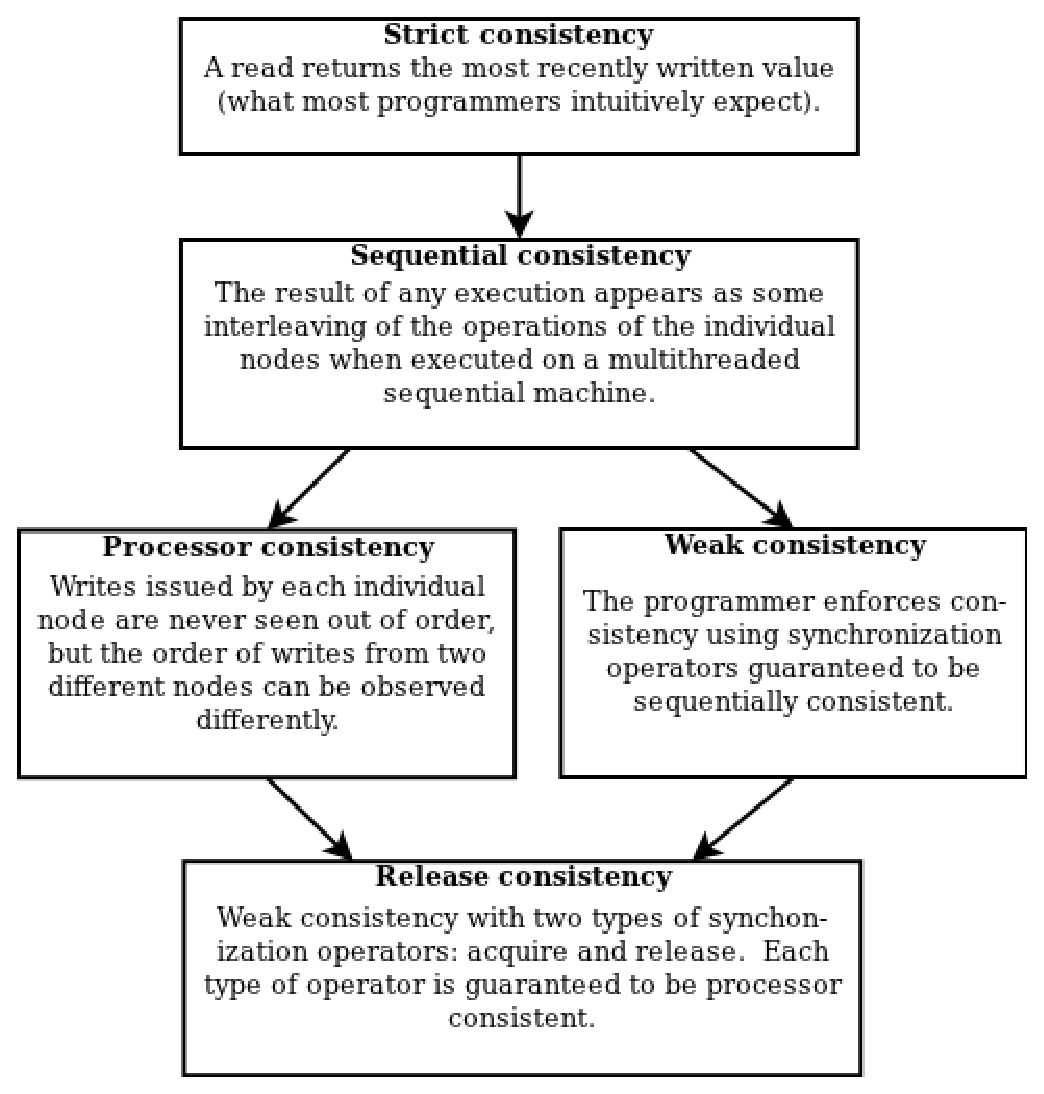
\includegraphics[scale=0.40]{images/memory_consistency.eps}
\caption{Intuitive definitions of memory coherence~\cite{Nitzberg:1991:DSM:112827.112855}.  The arrows point from stricter to weaker consistencies.}
\end{figure}

The remainder of this section depends on the following definitions of a memory access, originally defined by Debois in \cite{Scheurich:1987:CMO:30350.30377, Dubois:1986:MAB:17356.17406} and elaborated on in \cite{Gharachorloo:1990:MCE:325164.325102}.  In the following, $P_x$ refers to a processor $x$.

\begin{quote}
\begin{definition}[Performing a Memory Request]
A $LOAD$ by $P_i$ is considered \em performed with respect to \em $P_k$ at a point in time when the issuing of a $STORE$ to the same address by $P_k$ cannot affect the value returned by the $LOAD$.  A $STORE$ by $P_i$ is considered \em performed with respect to \em $P_k$ at a point in time when an issued $LOAD$ to the same address by $P_k$ returns the value defined by this $STORE$ (or a subsequent $STORE$ to the same location).  An access is \em performed \em when it is performed with respect to all processors.
\end{definition}
\end{quote}
\hfill \\

Additionally, a distinction between \em performed \em and \em globally performed \em $LOAD$ accesses is necessary for architectures with non-atomic $STORE$s.  A $STORE$ is atomic if the value stored becomes readable to all processors at the same time~\cite{Gharachorloo:1990:MCE:325164.325102}.  For DSM systems, it is typically not the case that $STORE$ operations are atomic unless special hardware is used.

\begin{quote}
\begin{definition}[Performing a $LOAD$ Globally]
A $LOAD$ is \em globally performed \em if it is performed \em and \em if the $STORE$ that is the source of the returned value has been performed.
\end{definition}
\end{quote}

\subsection{Strict Consistency}
In order to write programs that correctly execute on a platform, a programmer must understand the memory consistency protocols used on that platform.  The most intuitive protocol programmers expect to see in a platform is \em strict consistency\em~\cite{Goodman:1989:53705}.

As identified by Li and Hudak in \cite{Li:1989:MCS:75104.75105}, a memory is \em coherent \em if the value returned by a read operation is always the value written by the most recent write operation to the same address.  This definition of \em coherent \em memory is exactly what \em strict consistency \em guarantees: a memory read operation returns the most recently written memory value~\cite{Nitzberg:1991:DSM:112827.112855}.  This memory consistency model exhibits the most restrictive rules and serves as a base rule in many of Lamport's formalisms in \cite{Lamport:1979:MMC:1311099.1311750}.  However, because the restrictive rues oftentimes necessitate serial reading and writing, this coherency model is not used in DSM systems whose focus is speed or efficiency.

\subsection{Sequential Consistency}

On platforms with multiple execution paths (e.g., a multicore processor) programmers expect memory to be \em sequentially consistent\em.  In a \em sequentially consistent \em model, separate processors are expected to be \em strictly coherent\em, but the order of memory access between those processes is defined by the programmer.  A system is sequentially consistent if the result of any execution is the same as if the operations of all the processors were executed in some sequential order, and the operations of each individual process or appear in this sequence in the order specified by its program~\cite{Lamport:1979:MMC:1311099.1311750}.  Dubois studied how one may order events to guarantee sequential consistency in \cite{Scheurich:1987:CMO:30350.30377} by formally demonstrating that ordering $LOAD$ and $STORE$ in a fashion that prevents simultaneous access guarantees correct execution of an application program. 

\subsection{Processor Consistency}

Goodman in \cite{Goodman:1989:53705} introduced the concept of \em processor consistency \em to relax the ordering of \em sequential consistency\em.  Processor consistency requires that memory writes occur strictly consistent only on the executing processor.  To another processor the memory events need not occur in a strictly consistent manner.  Though this consistency model may yield incorrect if the programmer assumes a sequentially consistency, Goodman showed that most applications give the same results because explicit synchronization primitives are used~\cite{Goodman:1989:53705}.  This consistency model is used in combination with weak consistency models to synthesize release consistency models (discussed in Section \ref{release-consistency}).

\subsection{Weak Consistency}
\label{weak-consistency}

When discussing weaker consistency model the discussion is usually limited to two things: correctness and performance.  Correctness is important for showing a weaker consistency model is equivalent to a stricter consistency model in regards to a program's execution.  The main purpose of weaker coherency models is performance~\cite{Gharachorloo:1990:MCE:325164.325102}.  Weaker consistency models can be derived by grouping competing and synchronized memory requests to synchronization points in the program~\cite{Gharachorloo:1990:MCE:325164.325102}.  In practice, this means delaying the ordering of memory events to some synchronization point -- typically, a release or acquire.

This type of coherency protocol provides a sufficient programming environment for programs that require synchronization -- e.g., programs that require serial execution for critical sections and barriers~\cite{Steinke:2004:UTS:1017460.1017464} -- while maintaining a simple programming interface for developer.  Correctness of execution is so because the programmer is expected to coordinate when data may be accessed through synchronization primitives.  More concretely, if a program relies on critical sections to correctly execute, the programmer is responsible for ensuring that the memory written to by the critical sections is not read until all processors are done writing using synchronization primitives provided by the underlying system.

Additionally, it has also been shown in work such as \cite{Scheurich:1987:CMO:30350.30377} and \cite{Scales:1997:TTE:268998.266673} that these weaker consistency models can be implemented invisibility to the application programmer.  By implementing a compiler that invisibly enforces consistency rules, an application written to adhere to a processor consistency memory interface (e.g., written using synchronization primitives to ensure correctness of execution) can be further translated to work on a even weaker memory consistency model.  In the case of Shasta, application programs like Oracle 7.3 database system originally compiled for a single shared-memory multiprocessor were able to successfully run on this release consistent DSM system without any changes to the original application program~\cite{Scales:1997:TTE:268998.266673}.

Gharachorloo provided the following conditions for weak consistency in \cite{Gharachorloo:1990:MCE:325164.325102}:

\begin{quote}
\begin{condition}[Weak Consistency]
(A) before an ordinary $LOAD$ or $STORE$ access is allowed to perform with respect to any other processor, all previous \em synchronization \em accesses must be performed, and (B) before a \em synchronization \em access is allowed to perform with respect to any other processor, all previous ordinary $LOAD$ and $STORE$ accesses must be performed, and (C) \em synchronization \em accesses are sequentially consistent with respect to one another.
\end{condition}
\end{quote}

\subsection{Release Consistency}
\label{release-consistency}

Release consistency is a weak consistency model that further relaxes the restrictions of the consistency model discussed in Section \ref{weak-consistency} by overlapping release and acquire synchronization events.  This additional change differentiates synchronization and regular accesses to memory, which allow release consistent models to exploit access patterns to provide better performance.  This model effectively creates a pipeline of release and acquire events.

\begin{quote}
\begin{condition}[Release Consistency]
(A) before an ordinary $LOAD$ or $STORE$ access is allowed to perform with respect to any other processor, all previous \em acquire \em accesses must be performed, and (B) before a \em release \em access is allowed to perform with respect to any other processor, all previous ordinary $LOAD$ and $STORE$ accesses must be performed, and (C) \em special accesses \em are processor consistent with respect to one another.
\end{condition}
\end{quote}

\subsubsection{Eager \& Lazy Release Consistency}

Several other researchers have formalized the conditions for release consistency in works such as \cite{Gharachorloo:1990:MCE:325164.325102} and \cite{Keleher:1992:LRC:139669.139676}, which serve as a basis for other derived coherency models discussed later in this section:

The two main variants of release consistency in literature are \em eager release consistency \em and \em lazy release consistency\em.  These two coherency models are used by the major of software DSM systems, such as Treadmarks in \cite{Amza:1996:TSM:226705.226708,Keleher:1994:TDS:1267074.1267084}, Munin in \cite{Keleher:1992:LRC:139669.139676, Bennett:1990:MDS:99163.99182, Carter:1991:IPM:121132.121159, Zwaenepoel:1992:MDS:134397.135235} and Shasta in \cite{Scales:1996:SLO:237090.237179}.  Each of these derivatives obey the conditions for release consistency derived in \cite{Gharachorloo:1990:MCE:325164.325102}, but treat communication differently.  As the names suggest, \em eager release consistency \em communicate memory accesses as they happen, whereas \em lazy release consistency \em delays communication of memory accesses until some prescribed event occurs.

\paragraph{Eager Release Consistency (ERC)} ERC protocols delay propagating its modifications to shared data until a \em release \em synchronization access and is studied in \cite{Keleher:1992:LRC:139669.139676}.  At the time of a \em release\em, the ERC protocol propagates modifications to all other processors that cache the memory page.  A naive implementation of an ERC protocol may propagate these changes at the \em release \em or send invalidate requests to processors working on the memory page.  However, regardless of the implementation details of the ERC protocol, significant overhead is incurred by communicating changes at each \em release \em event.

\paragraph{Lazy Release Consistency (LRC)} LRC protocols delay propagating its modifications to shared data until an \em acquire \em synchronization access and is studied in \cite{Keleher:1992:LRC:139669.139676}.  At the time of an \em acquire\em, the LRC protocol propagates modifications to the requesting processor by piggybacking the changes to the memory page on a successful \em acquire \em message~\cite{Keleher:1992:LRC:139669.139676}.  Optimizations also exist that can allow an acquiring processor to only request changes that it actually needs.